\documentclass{Configuration_Files/PoliMi3i_thesis}

% CONFIGURATIONS
\usepackage{parskip} % For paragraph layout
\usepackage{setspace} % For using single or double spacing
\usepackage{emptypage} % To insert empty pages
\usepackage{multicol} % To write in multiple columns (executive summary)
\setlength\columnsep{15pt} % Column separation in executive summary
\setlength\parindent{0pt} % Indentation
\raggedbottom  

% PACKAGES FOR TITLES
\usepackage{titlesec}
% \titlespacing{\section}{left spacing}{before spacing}{after spacing}
\titlespacing{\section}{0pt}{3.3ex}{2ex}
\titlespacing{\subsection}{0pt}{3.3ex}{1.65ex}
\titlespacing{\subsubsection}{0pt}{3.3ex}{1ex}
\usepackage{color}

% PACKAGES FOR LANGUAGE AND FONT
\usepackage[english]{babel} % The document is in English  
\usepackage[utf8]{inputenc} % UTF8 encoding
\usepackage[T1]{fontenc} % Font encoding
\usepackage[11pt]{moresize} % Big fonts

% PACKAGES FOR IMAGES 
\usepackage{graphicx}
\usepackage{transparent} % Enables transparent images
\usepackage{eso-pic} % For the background picture on the title page
\usepackage{subfig} % Numbered and caption subfigures using \subfloat.
\usepackage{tikz} % A package for high-quality hand-made figures.
\usetikzlibrary{}
\graphicspath{{./Images/}} % Directory of the images
\usepackage{caption} % Coloured captions
\usepackage{xcolor} % Coloured captions
\usepackage{amsthm,thmtools,xcolor} % Coloured "Theorem"
\usepackage{float}

% STANDARD MATH PACKAGES
\usepackage{amsmath}
\usepackage{amsthm}
\usepackage{amssymb}
\usepackage{amsfonts}
\usepackage{bm}
\usepackage[overload]{empheq} % For braced-style systems of equations.
\usepackage{fix-cm} % To override original LaTeX restrictions on sizes

% PACKAGES FOR TABLES
\usepackage{tabularx}
\usepackage{longtable} % Tables that can span several pages
\usepackage{colortbl}

% PACKAGES FOR ALGORITHMS (PSEUDO-CODE)
\usepackage{algorithm}
\usepackage{algorithmic}

% PACKAGES FOR REFERENCES & BIBLIOGRAPHY
\usepackage[
	colorlinks=true,
	linkcolor=black,
	anchorcolor=black,
	citecolor=black,
	filecolor=black,
	menucolor=black,
	runcolor=black,
	urlcolor=black
]{hyperref} % Adds clickable links at references
\usepackage{cleveref}
\usepackage[square, numbers, sort&compress]{natbib} % Square brackets, citing references with numbers, citations sorted by appearance in the text and compressed
\bibliographystyle{abbrvnat} % You may use a different style adapted to your field

% OTHER PACKAGES
\usepackage{pdfpages} % To include a pdf file
\usepackage{afterpage}
\usepackage{lipsum} % Dummy package
\usepackage{fancyhdr} % For the headers
\usepackage{enumitem}
\fancyhf{}
\usepackage{listingsutf8}
\usepackage{xcolor}
\usepackage{pythonhighlight}

% Input of configuration file. Do not change config.tex file unless you really know what you are doing. 
% Define blue color typical of polimi
\definecolor{bluepoli}{cmyk}{0.4,0.1,0,0.4}

% Custom theorem environments
\declaretheoremstyle[
  headfont=\color{bluepoli}\normalfont\bfseries,
  bodyfont=\color{black}\normalfont\itshape,
]{colored}

% Set-up caption colors
\captionsetup[figure]{labelfont={color=bluepoli}} % Set colour of the captions
\captionsetup[table]{labelfont={color=bluepoli}} % Set colour of the captions
\captionsetup[algorithm]{labelfont={color=bluepoli}} % Set colour of the captions

\theoremstyle{colored}
\newtheorem{theorem}{Theorem}[chapter]
\newtheorem{proposition}{Proposition}[chapter]

% Enhances the features of the standard "table" and "tabular" environments.
\newcommand\T{\rule{0pt}{2.6ex}}
\newcommand\B{\rule[-1.2ex]{0pt}{0pt}}

% Pseudo-code algorithm descriptions.
\newcounter{algsubstate}
\renewcommand{\thealgsubstate}{\alph{algsubstate}}
\newenvironment{algsubstates}
  {\setcounter{algsubstate}{0}%
   \renewcommand{\STATE}{%
     \stepcounter{algsubstate}%
     \Statex {\small\thealgsubstate:}\space}}
  {}

% New font size
\newcommand\numfontsize{\@setfontsize\Huge{200}{60}}

% Title format: chapter
\titleformat{\chapter}[hang]{
\fontsize{50}{20}\selectfont\bfseries\filright}{\textcolor{bluepoli} \thechapter\hsp\hspace{2mm}\textcolor{bluepoli}{|   }\hsp}{0pt}{\huge\bfseries \textcolor{bluepoli}
}

% Title format: section
\titleformat{\section}
{\color{bluepoli}\normalfont\Large\bfseries}
{\color{bluepoli}\thesection.}{1em}{}

% Title format: subsection
\titleformat{\subsection}
{\color{bluepoli}\normalfont\large\bfseries}
{\color{bluepoli}\thesubsection.}{1em}{}

% Title format: subsubsection
\titleformat{\subsubsection}
{\color{bluepoli}\normalfont\large\bfseries}
{\color{bluepoli}\thesubsubsection.}{1em}{}

% Shortening for setting no horizontal-spacing
\newcommand{\hsp}{\hspace{0pt}}

\makeatletter
% Renewcommand: cleardoublepage including the background pic
\let\cleardoublepage\clearpage

%For correctly numbering algorithms
\numberwithin{algorithm}{chapter}

%----------------------------------------------------------------------------
%	BEGIN OF YOUR DOCUMENT
%----------------------------------------------------------------------------

\begin{document}

\fancypagestyle{plain}{%
\fancyhf{} % Clear all header and footer fields
\fancyhead[RO,RE]{\thepage} %RO=right odd, RE=right even
\renewcommand{\headrulewidth}{0pt}
\renewcommand{\footrulewidth}{0pt}}

%----------------------------------------------------------------------------
%	TITLE PAGE
%----------------------------------------------------------------------------

\pagestyle{empty} % No page numbers
\frontmatter % Use roman page numbering style (i, ii, iii, iv...) for the preamble pages

\puttitle{
	title={IoT Challenge \#1,\\Wokwi and Power Consumption},% Title of the thesis
	course={Internet of Things},
	name1={Kevin Ziroldi - 10764177},
	name2={Matteo Volpari - 10773593},
	advisors= {Alessandro Redondi, Antonio Boiano}, % Supervisor name
	academicyear={2024-2025},  % Academic Year
	version={1.0}, 
	releasedate={20-3-2025}
} 
          
%----------------------------------------------------------------------------
%	PREAMBLE PAGES: ABSTRACT (inglese e italiano), EXECUTIVE SUMMARY
%----------------------------------------------------------------------------
\startpreamble
\setcounter{page}{1} % Set page counter to 1

%----------------------------------------------------------------------------
%	LIST OF CONTENTS/FIGURES/TABLES/SYMBOLS
%----------------------------------------------------------------------------

% TABLE OF CONTENTS
\thispagestyle{empty}
\tableofcontents % Table of contents 
\thispagestyle{empty}
\cleardoublepage

%-------------------------------------------------------------------------
%	THESIS MAIN TEXT
%-------------------------------------------------------------------------
% In the main text of your thesis you can write the chapters in two different ways:
%
%(1) As presented in this template you can write:
%    \chapter{Title of the chapter}
%    *body of the chapter*
%
%(2) You can write your chapter in a separated .tex file and then include it in the main file with the following command:
%    \chapter{Title of the chapter}
%    \input{chapter_file.tex}
%
% Especially for long thesis, we recommend you the second option.

% The \label{...}% enables to remove the small indentation that is generated, always leave the % symbol.

\addtocontents{toc}{\vspace{2em}} % Add a gap in the Contents, for aesthetics
\mainmatter % Begin numeric (1,2,3...) page numbering

% --------------------------------------------------------------------------
% NUMBERED CHAPTERS % Regular chapters following
% --------------------------------------------------------------------------

\chapter{Code explanation}
\label{ch:CodeExplanation}%
In this section, we will describe the main structure of the code written to meet the specification provided to us.
\section{Global variables}
\subsection{Auxiliary variables}
We have defined two global variables that are not strictly necessary for the correct operation of the system but are useful for future points of the challenge.
\begin{verbatim}
#define DEBUG 0
\end{verbatim}
Variable which, when set to 1, is used in testing to print the messages arriving in broadcast to the board and the status of the messages sent. This variable also introduces a small delay of 10 ms to print the messages before going into deep sleep.\\
\begin{verbatim}
#define TIME_MEASUREMENT 1
\end{verbatim}
This variable, when set to 1, is used to measure all the inter-times of the various phases of a system operation cycle. To function correctly, \textit{DEBUG} must be set to 0, otherwise the data collected is distorted by the delay introduced by \textit{DEBUG}.


\subsection{Pin declaration}
\begin{verbatim}
#define TRIG 4
#define ECHO 2
\end{verbatim}
We have defined 2 variables which identify the functional pins used by HC-SR04 sensor and which we have connected to pins 4 and 2 of the ESP32 board.

\subsection{Exercise constants}
\begin{verbatim}
#define TIME_TO_SLEEP 48
\end{verbatim}
Variable used to define the time for which the board will go into deep sleep. The value 48 is calculated using the formula: \textit{TIME\_TO\_SLEEP} = 93\%50+5 = 48 \\
where 93 is coming from the person code 10773593. \\
\begin{verbatim}
#define uS_TO_S_FACTOR 1000000
\end{verbatim}
Constant equal to $10^6$ used to convert from seconds to $\mu\text{s}$.\\
\begin{verbatim}
#define DISTANCE_LIMIT 50
\end{verbatim}
Threshold distance of 50 cm set by the exercise to consider the parking space occupied or not.


\section{Auxiliary functions}
We have used various auxiliary functions to make the code more readable and functional, which we will describe in this section.\\
\begin{verbatim}
void setupESP_NOW()
\end{verbatim}
This function is used to switch on the WiFi and do the setup.
In the setup phase, we set the transmission power to 2 dBm and assign two callback functions which are used during debugging and triggered when messages are sent or received (\textit{OnDataSent} and \textit{OnDataRecv}). \\
\begin{verbatim}
void OnDataSent(const uint8_t *mac_addr, esp_now_send_status_t status)
void OnDataRecv(const uint8_t * mac, const uint8_t *data, int len) 
\end{verbatim}
These are two callback functions which are used in debugging to print out whether a message has been sent correctly or whether there have been errors and all messages arriving on the board. \\
\begin{verbatim}
float getDistanceSensorMeasurement()
\end{verbatim}
This function is used to perform a single measurement via the ultrasonic sensor.
The measurement is made by setting the trig pin to high, after which a delay of 10 $\mu\text{s}$ is waited and the value of the trig pin is reset to low. \\
The delay is required by the HC-SR04 component specification, which needs the \textit{TRIG} pin to remain high for at least 10 $\mu\text{s}$ in order to make a measurement. After taking the data it converts it into cm and returns it.

\section{Setup function}
The setup function is the heart of the system and is executed by the board every time it wakes up. In our implementation, the setup contains all the actions performed by the board, since the loop is empty. We have chosen not to use the loop function because, after being sent into deep sleep, the board will have to start over from setup.\\
First of all, the setup function sets the data rate for serial data transmission to write to the serial.
Then, the modes of the two pins \textit{TRIG} and \textit{ECHO} are set to output and input respectively.
After this, a measurement is made via the ultrasonic sensor and, only then, the \textit{setupESP\_NOW()} function is called to activate WiFi.\\
When the WiFi is switched on and ready to be used, a message is sent to the MAC address of the sink, which in this case is set to the broadcast address 8C:AA:B5:84:FB:90.\\
Once the measurement is sent, the WiFi is switched off to reduce the energy consumption and the system is sent into deep sleep.
On awakening from deep sleep, the board will restart from the beginning of the setup function and will then perform all the operations already seen in the same order.\\








\chapter{Energy consumption estimation}
\label{ch:EnergyConsumptionEstimation}%
\section{Power consumption estimation}
In this section, there is a description of the power consumption of the ESP32 node in all states: deep sleep, idle, sensor reading, WiFi turned on and transmission.\\
In order to estimate power consumption based on the provided CSV files, we first plotted data using Python and Matplotlib library. Based on the plot, we computed the average power consumption in the analyzed working state.

\subsection{Power consumption plots}
In order to plot the data contained in the provided CSV files, we used the following algorithm.

\begin{python}
import pandas as pd
import matplotlib.pyplot as plt
# read CSV file 
df = pd.read_csv('deep_sleep.csv', parse_dates=['Timestamp'])
# plot data
plt.figure(figsize=(10, 6))
plt.plot(df['Timestamp'], df['Data'], linestyle='-', linewidth=2)
plt.xlabel('Time')
plt.ylabel('Power [mW]')
plt.title('Power consumption deep sleep')
plt.grid(True)
# save and shows
plt.savefig("power_consumption_deep_sleep.pdf", format="pdf", bbox_inches="tight")
plt.show()
\end{python}

\subsubsection{Power consumption deep\_sleep.csv}
The following plot represents the power consumption when the ESP32 is in deep sleep state (lowest power level), goes into idle mode (medium power level) and finally turns the WiFi on (highest power level). 
\begin{figure}[H]
    \centering
    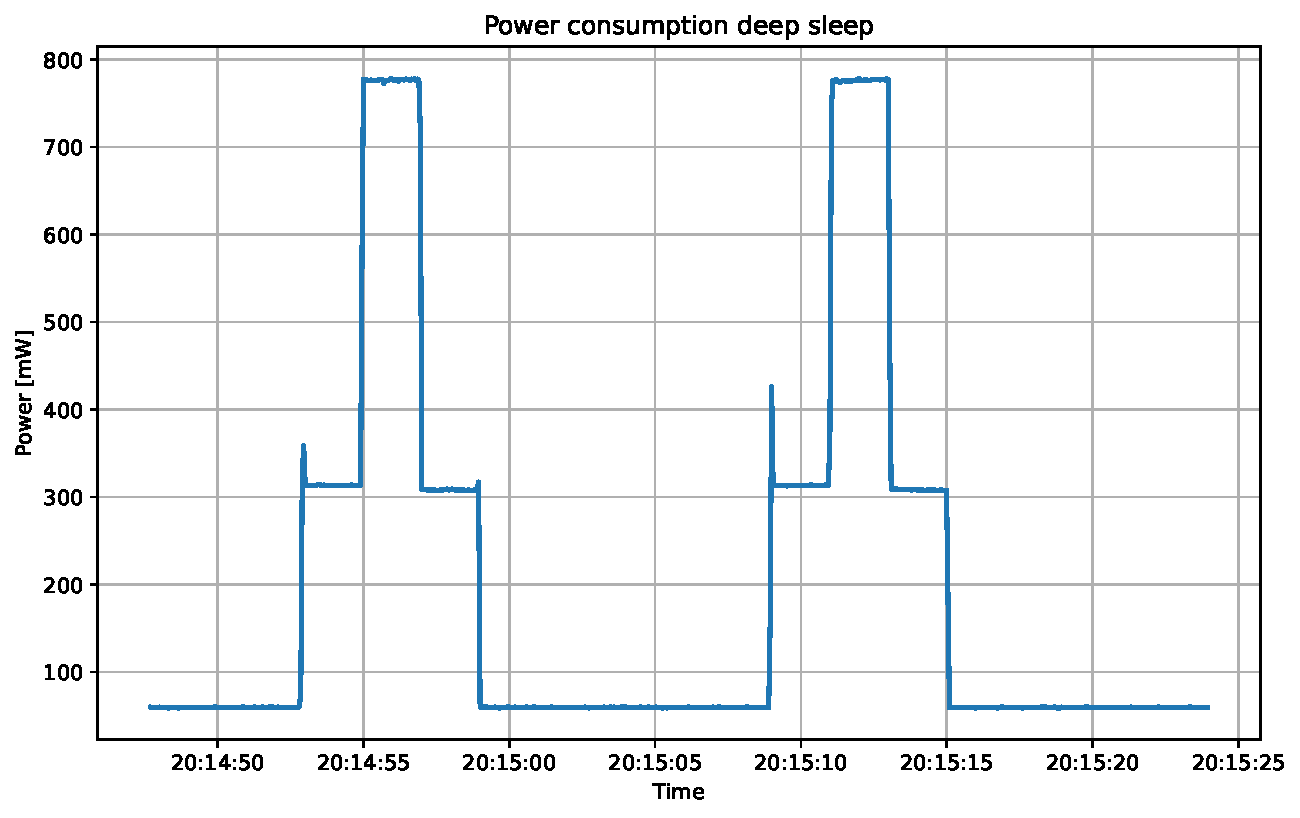
\includegraphics[width=\linewidth, height=0.4\textheight, keepaspectratio]{power_consumption_deep_sleep.pdf}
    \caption{Power consumption deep sleep state}
    \label{fig:Power consumption deep sleep state}
\end{figure}

\subsubsection{Power consumption sensor\_read.csv}
The following plot represents the power consumption when the ESP32 alternates the idle mode and sensor reading mode, in which it performs a measurement using the ultrasonic distance sensor HC-SR04.
\begin{figure}[H]
    \centering
    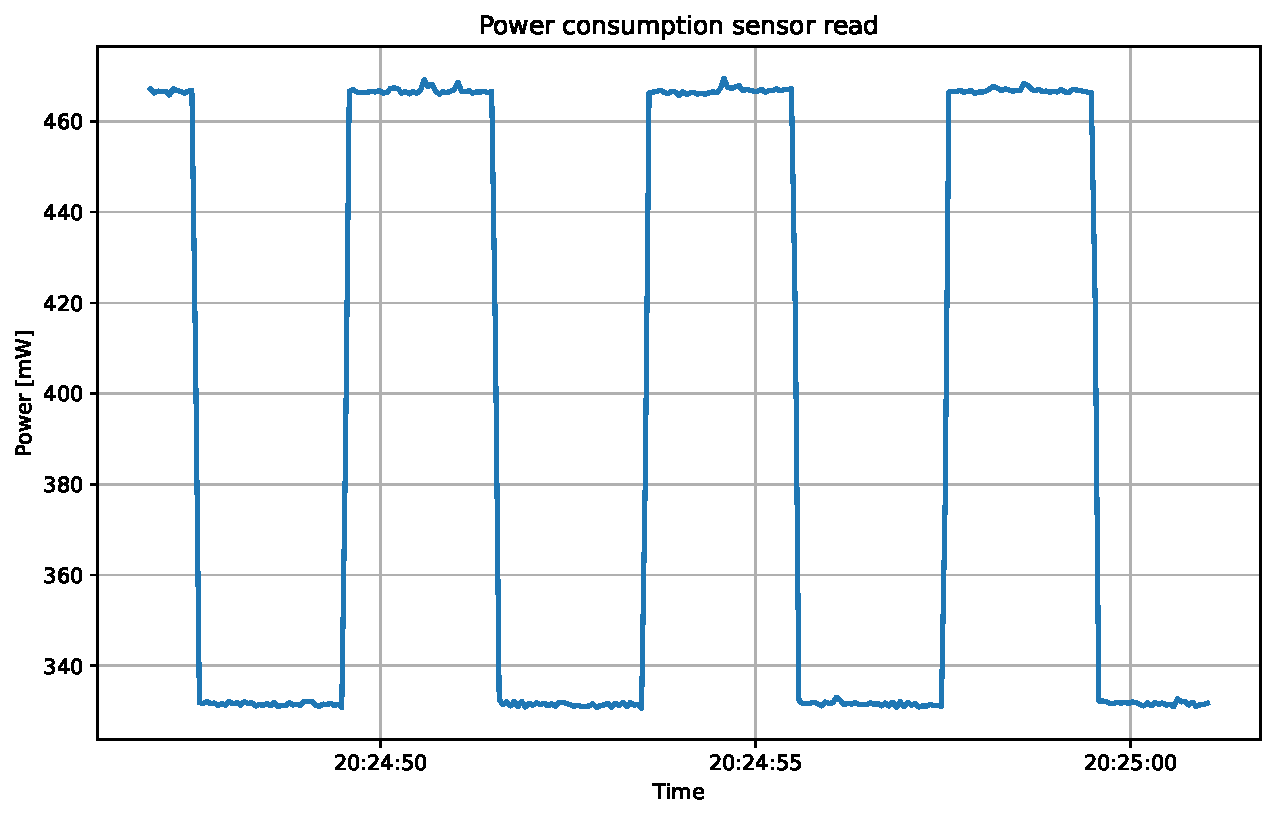
\includegraphics[width=\linewidth, height=0.4\textheight, keepaspectratio]{power_consumption_sensor_read.pdf}
    \caption{Power consumption deep sleep state}
    \label{fig:Power consumption deep sleep state}
\end{figure}

\subsubsection{Power consumption transmission\_power.csv}
The following plot represents the power consumption when the ESP32 has the WiFi turned on and transmits data using ESP-NOW at 19.5 dBm and 2 dBm.
\begin{figure}[H]
    \centering
    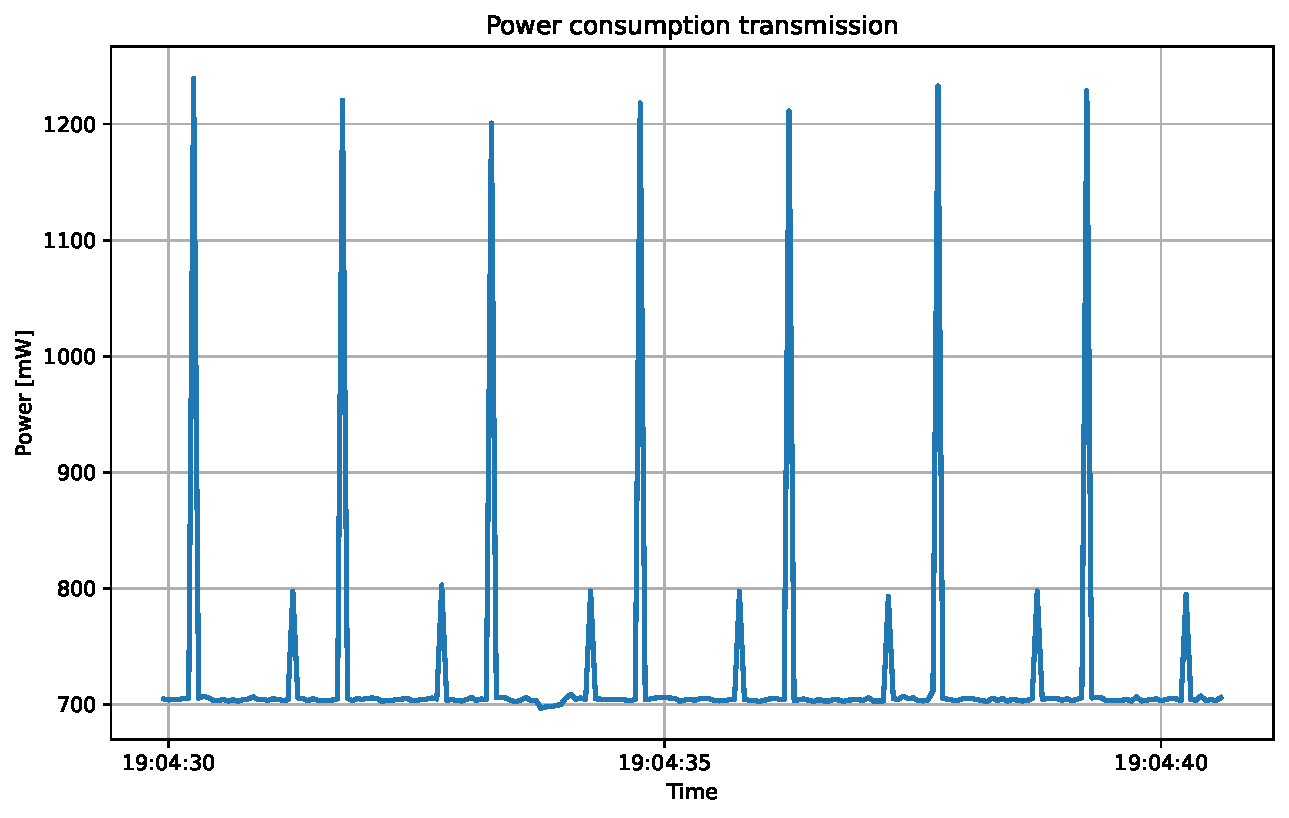
\includegraphics[width=\linewidth, height=0.4\textheight, keepaspectratio]{power_consumption_transmission.pdf}
    \caption{Power consumption deep sleep state}
    \label{fig:Power consumption deep sleep state}
\end{figure}

\subsection{Average power consumption values}
In order to find a numerical estimation of the power consumption in different states, we used some Python algorithms, using the library Pandas. Starting from the plot we selected the range of values regarding a particular state, discarding the others, and computed the average power consumption. For some states, the values of power can be found in multiple CSV files; in such cases, we merged different files in order to have a more accurate estimation.\\
In the following sections we also report two example of algorithms used to compute the average, both using a single dataset and multiple datasets.

\subsubsection{Power consumption in deep sleep state}
Data to estimate the deep sleep mode is contained in the dataset deep\_sleep.csv. We filtered all values of power above 100mW, referring to other states as shown by the plot, and computed the average.

\begin{python}
import pandas as pd 
# read CSV file 
dataset_deep_sleep = pd.read_csv("deep_sleep.csv", parse_dates=['Timestamp'])
# filter data with power < 100mW, referring to deep sleep mode
deep_sleep_data = dataset_deep_sleep[dataset_deep_sleep["Data"] < 100]
# compute average
deep_sleep_avg_power = deep_sleep_data["Data"].mean()
# print average 
print("Average power consumption deep sleep: ", deep_sleep_avg_power)
\end{python}

We obtained an average consumption in deep sleep of 59.66 mW.

\subsubsection{Power consumption in idle state}
The power consumption in idle state can be extracted both by sensor\_read.csv and transmission\_power.csv. We used both datasets, merging all values and computing the average. We considered only values between 200 mW and 500 mW, that refer to idle mode.
\begin{python}
import pandas as pd 
# read CSV file 
dataset_deep_sleep = pd.read_csv("deep_sleep.csv", parse_dates=['Timestamp'])
dataset_sensor_reading = pd.read_csv("sensor_read.csv", parse_dates=['Timestamp'])
# filter data with power between 200 mW and 500 mW, referring to idle mode
idle_data_deep_sleep = dataset_deep_sleep[(dataset_deep_sleep['Data'] >= 200) & (dataset_deep_sleep['Data'] <= 500)]
# filter data with power <= 400 mW, reffering to idle mode
idle_data_sensor_reading = dataset_sensor_reading[dataset_sensor_reading['Data'] <= 400]
# merge values 
idle_merged = pd.concat([idle_data_deep_sleep, idle_data_sensor_reading], ignore_index=True)
# compute average
idle_avg_power = idle_merged['Data'].mean()
# print average 
print("Average power consumption idle: ", idle_avg_power)
\end{python}

We obtained an average consumption in idle of 322.62 mW.

\subsubsection{Power consumption in measurement state}
Data representing power consumption in measurement state is contained in the dataset sensor\_read.csv. We computed the average value considering values of power above 400 mW and obtained an average value of 465.18 mW. The algorithm is very similar to deep sleep mode, thus we don't report it.

\subsubsection{Power consumption in WiFi on state}
We estimated the power consumption when the WiFi is turned on and the ESP32 is not transmitting based on deep\_sleep.csv and transmission\_power.csv, merging all value between 600 mW and 750 mW, as shown for the idle mode. The average power consumption when WiFi is turned on is 724.58 mW.

\subsubsection{Power consumption when transmitting at 2 dBm}
Finally, we estimated the average power consumption when ESP32 is transmitting at 2 dBm, based on transmission\_power.csv. We compute the average of values between 750 mW and 900 mW, obtaining an average value of 797.29 mW.

\subsubsection{Summary power consumption}
The summary of power consumption of ESP32 in different states is reported below.

\begin{table}[H]
\centering 
\begin{tabular}{| c | c |}
	\hline 
	\rowcolor{bluepoli!40}
	\textbf{State} & \textbf{Power}\T\B \\
	\hline 
	$P_{idle}$ & $322.62\,\text{mW}$ \T\B\\
	$P_{measurement}$ & $465.18\,\text{mW}$ \T\B\\
	$P_{WiFi}$ & $724.58\,\text{mW}$ \T\B\\
	$P_{transmission}$ & $797.29\,\text{mW}$ \T\B\\
	$P_{deep\_sleep}$  & $59.66\,\text{mW}$ \T\B\\
	\hline
\end{tabular}
\\[10pt]
\caption{States power table}
\label{table:states_power_table}
\end{table}

\section{States duration estimation}
We estimated the duration of different states by simulating the ESP32 on Wokwi and measuring them. We saved the timestamps in different points of execution, computed the duration of each state and printed it on the serial log.\\
We simulated the execution for about a hundred cycles and saved the serial log. We provide few examples of entries of the serial log, in which the durations are in microseconds.

\begin{verbatim}
entry 0x400805dc
Idle duration: 882
Measurement duration: 24116
Sending duration: 64
WiFi duration: 189158
ets Jul 29 2019 12:21:46

entry 0x400805dc
Idle duration: 846
Measurement duration: 24212
Sending duration: 65
WiFi duration: 188548
ets Jul 29 2019 12:21:46

entry 0x400805dc
Idle duration: 845
Measurement duration: 24211
Sending duration: 64
WiFi duration: 187548
ets Jul 29 2019 12:21:46
\end{verbatim}

We computed the duration of different states using a Python algorithm to extract the values from the log, using regexes, filtering outliers and computing the average. \\
In the measurement of the sending duration, during which the ESP32 uses WiFi, we noticed the presence of some values completely different from the others, caused by the simulation on Wokwi; we filtered them out to get a more accurate estimation. \\
Finally, we observed that the duration of the measurement with the HC-SR04 ultrasonic distance sensor varies based on the resulting distance: the higher the distance, the longer the duration. In order to have a realistic duration, we gathered data with different values of measured distance.

\begin{python}
import re
import statistics
# open log file
with open("time_measurements_log.txt", "r") as file:
    log_text = file.read()
# extract values from log using a regex 
idle_values = list(map(int, re.findall(r"Idle duration:\s*(\d+)", log_text)))
measurement_values = list(map(int, re.findall(r"Measurement duration:\s*(\d+)", log_text)))
sending_values = list(map(int, re.findall(r"Sending duration:\s*(\d+)", log_text)))
wifi_values = list(map(int, re.findall(r"WiFi duration:\s*(\d+)", log_text)))
# filter wrong values, given by the simulation
wifi_values = [value for value in wifi_values if value <= 200000]
# compute averages
avg_idle = statistics.mean(idle_values) if idle_values else 0
avg_measurement = statistics.mean(measurement_values) if measurement_values else 0
avg_sending = statistics.mean(sending_values) if sending_values else 0
avg_wifi = statistics.mean(wifi_values) if wifi_values else 0
#print values
print("Average Idle duration:", avg_idle)
print("Average Measurement duration:", avg_measurement)
print("Average Sending duration:", avg_sending)
print("Average WiFi duration:", avg_wifi)
\end{python}

The deep sleep duration is computed from the last two digits of the person code, 10773593, as:
\begin{align*}
	T_{deep\_sleep} &= (93 \% 50) + 5 = 48\,\text{s} \\ 
\end{align*}

The duration of different states is reported in the following table.

\begin{table}[H]
\centering 
\begin{tabular}{| c | c |}
	\hline 
	\rowcolor{bluepoli!40}
	\textbf{State} & \textbf{Duration}\T\B \\
	\hline 
	$T_{idle}$ & $833.70\,\mu\text{s}$ \T\B\\
	$T_{measurement}$ & $18647.79\,\mu\text{s}$ \T\B\\
	$T_{WiFi}$ & $188640.86\,\mu\text{s}$ \T\B\\
	$T_{transmission}$ & $59.60\,\mu\text{s}$ \T\B\\
	$T_{deep\_sleep}$  & $48\times10^6\,\mu\text{s}$ \T\B\\
	\hline
\end{tabular}
\\[10pt]
\caption{States duration table}
\label{table:states_duration_table}
\end{table}

\section{Energy consumption estimation}
Starting from the power consumption and states durations estimations, we can easily compute energy consumed by the ESP32 by multiplying the power and the time of each state.\\
At start, the ESP32 is in idle mode for T\_{idle}. Then it enters measurement mode to measure the distance with the ultrasonic distance sensor HC-SR04 for T\_{measurement}. When the measurement is completed, the ESP32 turns the WiFi on for T\_{WiFi} and, during this same period, it transmits data at 2 dBm for T\_{transmission}. Finally, it enters deep sleep for T\_{deep\_sleep}. \\

The energy for different states is computed as follows.
\begin{align*}
	E_{idle} &= P_{idle} \cdot T_{idle} = 0.268 \,\text{mJ} \\ 
	E_{measurement} &= P_{measurement} \cdot T_{measurement} = 8.675 \,\text{mJ} \\
	E_{WiFi} &= P_{WiFi} \cdot \Bigl(T_{WiFi} - T_{transmission} \Bigr) = 136.642\,\text{mJ} \\
	E_{transmission} &= P_{transmission} \cdot T_{transmission} = 0.048\,\text{mJ} \\
   	E_{deep\_sleep} &= P_{deep\_sleep} \cdot T_{deep\_sleep} = 2863,680\,\text{mJ} 
\end{align*}

The energy consumption for a cycle is computed as the sum.
\[
E_{cycle} = E_{idle} + E_{measurement} + E_{WiFi} + E_{transmission} + E_{deep\_sleep} = 3009,313\,\text{mJ} 
\]

The available energy is computed from the last four digits of the person code, 10773593, as: 
\begin{align*}
	E_{b} &= (3593 \% 5000) + 15000 = 18593\,\text{J} = 18593000\,\text{mJ}
\end{align*}

The sensor node has a lifetime, measured in cycles, of:
\begin{align*}
	L_{cycles}&= E_{b}/E_{cycle} = 6178.487 \,\text{cycles} 
\end{align*}

The total time for a cycle is:
\begin{align*}
	T_{cycle} &= T_{idle} + T_{measurement} + T_{WiFi} + T_{deep\_sleep} = 48.208 \text{s}
\end{align*}

The lifetime, measured in time, is of:
\begin{align*}
	L_{time}&= L_{cycles} \cdot T_{cycle} = 297852.501 \text{s}
\end{align*}

The lifetime is equivalent to 3 days, 10 hours, 44 minutes and 12 seconds.


COORDINATES
6.87168 7.65929 8.15501




\chapter{Energy consumption improvements}
\label{ch:Improvements}%
In order to improve the energy consumption of this IoT system, it is possible modify multiple parameters:
\begin{itemize}
	\item transmission power for ESP-NOW communication;
	\item delay used to make a measurement with HC-SR04;
	\item time spent with WiFi turned on;
	\item time spent in deep sleep.
\end{itemize}

\section{Improvements for our implementation}
In our implementation, we use the lowest transmission power, of 2 dBm, and the lowest time, suggested by the documentation, of 10 $\mu \text{s}$ to make measurement with HC-SR04 ultrasonic sensor. Finally, we perform the board setup and the measurement with WiFi turned off.\\
Thus, the only parameter which we can modify to improve the system's lifetime is the deep sleep time. If we increased the time spent by the node in deep sleep, we would achieve a better lifetime, but we would need to tolerate a longer time to update the status of occupancy of the parking spot.\\
An alternative approach, consists in varying the frequency with which the node sends updates to the sink based on how the status of occupancy changes. If the status has changed over the last cycle, the node immediately notifies the sink; but, if the status doesn't change for a long time, the node can skip up to five transmission to the sink. If up to five transmissions are skipped, the sink can assume the occupancy value has not changed; after the fifth skipped transmission, the node notifies the sink with the occupancy value, which can be the same as the last one it sent, to inform it is still alive.\\
Thanks to this approach, when the status doesn't change, the node performs a measurement, computes the measured value and goes to deep sleep, instead of turning the WiFi on and transmitting data to the sink. Since the transmission represents a big part of the energy consumption of the node, we can increase the efficiency by a lot, without increasing the time needed to notify an update to the sink.\\

The power consumption of the ESP32 when the occupancy value doesn't changes is represented in the following plot.
\begin{figure}[H]
    \centering
    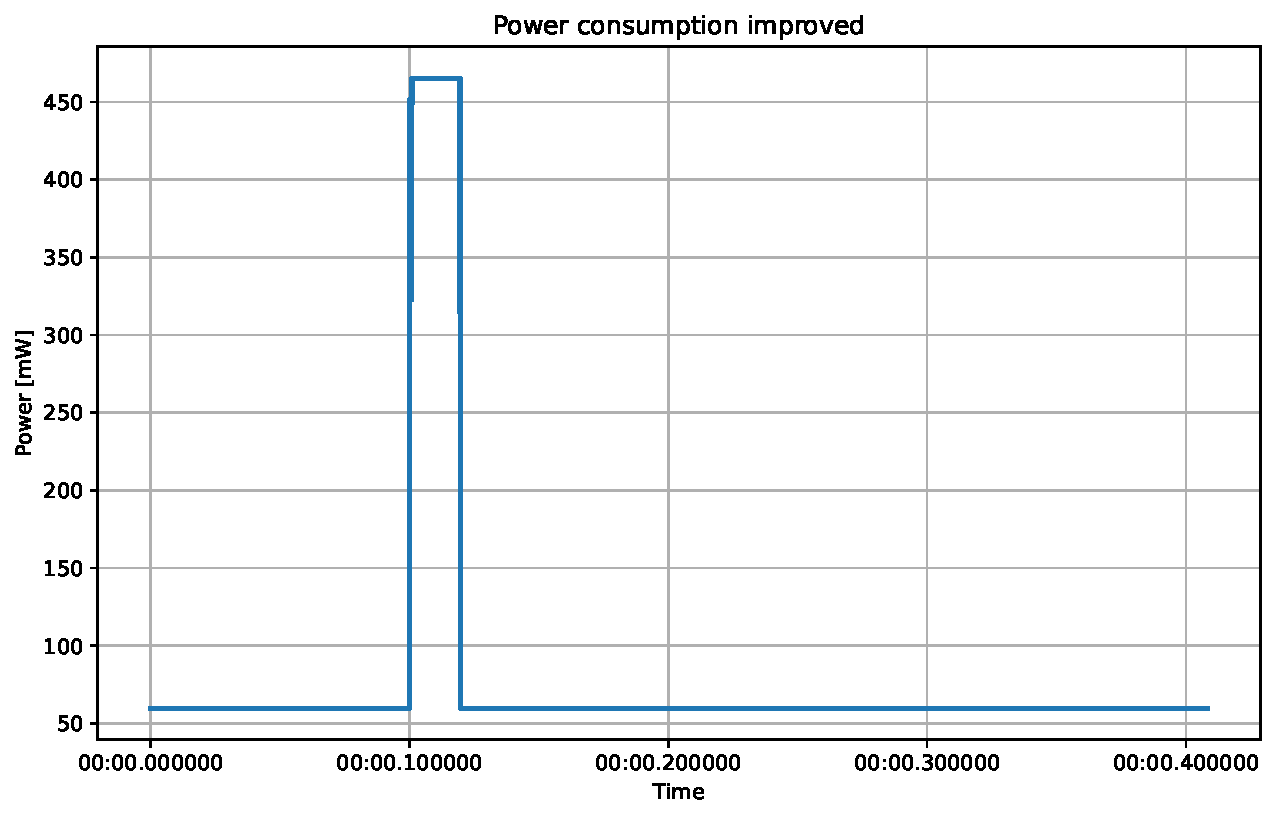
\includegraphics[width=\linewidth, height=0.4\textheight, keepaspectratio]{power_consumption_improved.pdf}
    \caption{Power consumption cycle without transmission}
    \label{fig:Power consumption cycle without transmission}
\end{figure}

We now compute the energy consumption of the node when the measurement doesn't change for 6 cycles, i.e. the ESP32 doesn't notify the sink for 5 times, since the measurement didn't change. This assumption looks reasonable, since this would mean that the occupancy of the parking spot, in the average situation, doesn't change more than one time every 5 minutes.\\
We compute the energy consumption for a cycle when the node doesn't notify the sink as:
\begin{align*}
E_{cycle}' = E_{idle} + E_{measurement} + E_{deep\_sleep}'
\end{align*}
Since we want to maintain a constant time for a cycle, the time spent in deep sleep is slightly higher, and can be computed as:
\begin{align*}
	T_{deep\_sleep}' = T_{cycle} - T_{idle} - T_{measurement} = 48.189 \text{s}\\
\end{align*}
The new energy consumption in deep sleep is:
\begin{align*}
	E_{deep\_sleep}' &= P_{deep\_sleep} \cdot T_{deep\_sleep}' = 2874.956\,\text{mJ} 
\end{align*}

Since the other values of energy consumptions are unchanged, we can compute the energy consumption of a cycle as:
\begin{align*}
	E_{cycle}' = E_{idle} + E_{measurement} + E_{deep\_sleep}' = 2883.899\,\text{mJ} 
\end{align*}
The energy consumption for 6 cycles, in which only one transmission is made is:
\begin{align*}
	E_{6\_cycles} = E_{cycle} + 5 \cdot E_{cycle}' = 17428.808\,\text{mJ} 
\end{align*}

The new sensor node's lifetime, measured in cycles, is:
\begin{align*}
	L_{cycles}&= 6 \cdot E_{b} / E_{6\_cycles} = 6400.782 \,\text{cycles} 
\end{align*}
The sensor will perform 6400 complete cycles and will die during the following one.

The total time for a cycle is always the same, $T_{cycle} = 48.208 s$, so the lifetime measured in time is of:
\begin{align*}
	L_{time}&= L_{cycles} \cdot T_{cycle} = 308568.899 \text{s}
\end{align*}

The new lifetime is equivalent to 3 days 13 hours 42 minutes and 48 seconds, which is more 3 hours longer than the base case.

\section{Improvements upper bound}
In order to put into perspective the energy efficiency of our system, we provide a theoretical upper bound of the system's lifetime, i.e. the lifetime when the deep sleep time tends toward infinity, the node always stays in deep sleep and isn't functional anymore.\\
The power consumption of the ESP32 in deep sleep mode is $P_{deep\_sleep} = 59.66\,\text{mW}$ and the battery life is $E_{b} = 18593\,\text{J}$, so the lifetime is:
\begin{align*}
	L_{time}&= E_{b} / P_{deep\_sleep} = 311649.346 \text{s}
\end{align*}

The lifetime of the system, when the deep sleep time tend towards infinity, is of 3 days 14 hours 34 minutes and 9 seconds, which is less than one our bigger than the improved version of the system.










%-------------------------------------------------------------------------
%	BIBLIOGRAPHY
%-------------------------------------------------------------------------

\addtocontents{toc}{\vspace{2em}} % Add a gap in the Contents, for aesthetics
\bibliography{Thesis_bibliography} % The references information are stored in the file named "Thesis_bibliography.bib"

%-------------------------------------------------------------------------
%	APPENDICES
%-------------------------------------------------------------------------

\end{document}

